\subsection{Jet Energy Scale Uncertainty}

The effect of the uncertainty in the JES, explained in Section \ref{sec:Det:Jets}, is studied using the reconstructed PYTHIA samples.
Each jet, which is at the central value of the JES by default, is shifted up and down by 1 standard deviation of the uncertainty on the JES.
The events are then passed through the event selection and three sets of the final distributions are made corresponding to nominal JES,  JES shifted up and JES shift down.
The JES uncertainty band was found by taking the ratio of the shifted distribution to the nominal distribution.


Figures \ref{GBJ2:JES:gap_njets} - \ref{GBJ2:JES:Q0} show the JES uncertainty bands for the final distributions.
The JES uncertainty shifting has two main effects that will apply differently in different distributions, one shifting the leading jet energy, and the other shifting the non-leading jets.
The shift in the leading jets energy has the effect of moving events across the \pt{} cuts at 60 GeV and 50 GeV.
This results in more events for JES shifted up and less events for JES shifted down. 
The effect of shifting the non-leading jets is mainly due to the shift in \pt{} of the highest \pt{} jet in the rapidity region bounded by the dijet system. 
This will affect distributions that probe non-leading jets, such as gap fraction or average number of jets. 

The JES uncertainty band for the gap fraction as a function of \dy{} is shown in Figure \ref{GBJ2:JES:gap_njets} (a), and is small for low \dy{}, but increases at larger \dy{}.
The effect of shifting the JES up for the leading jets is to include dijet events that have a lower \ptb{}. 
As seen in the previous analysis (Figure \ref{GBJ1:pTSelA}), dijets with lower \ptb{} have a higher gap fraction, and so the effect of the upwards shift is to increase the gap fraction.
Shifting the JES up of the non-leading jets increase the probability that there is a jet with $\pt{}>Q_0$ in the rapidity region, and so decreases the gap fraction. 
At low \dy{} the the effect is small and the two effects cancel.
At higher \dy{} the leading jets are more likely to be at a higher rapidity where the JES uncertainty is higher, the effects no longer cancel and the gap fraction increases.
Figure \ref{GBJ2:JES:gap_njets} (b) shows the JES uncertainty band for the average number of jets in the rapidity region and the overall uncertainty is approximately constant at $\pm 10 \%$.


Figure \ref{GBJ2:JES:dPhi} shows the JES uncertainty bands for \dphiDist{} for both the inclusive and gap events, for the different \dy{} ranges.
The uncertainty bands for \dphiDist{} are significantly larger than for other distributions, with $20-30\%$ uncertainty for the $2<\dy{}<3$ and $4<\dy{}<5$, and up to $70\%$ uncertainty for $7<\dy{}<8$ in the lowest \dphi{} bin.
The reason that the JES shifting effects the \dphiDist{} more than the gap fraction or average number of jets is due to the steepness of the curves in \ptb{}.
The shape of gap fraction and average number of jets against \ptb{} is relatively flat compared to the steeply falling cross-section against \ptb{}, and so there is more migration across the \pt{} cut causing the JES smearing to have larger effect on the cross-section. 
%The gap fraction and average number of jets distributions have a smaller effect because they are fractions and the increase in number of events due to the migration over the \pt{} cut effects both the numerator and denominator, and so the effects are partially cancelled. 
%However this is not the case with a cross-section. 
For the $2<\dy{}<3$ and $4<\dy{}<5$ ranges, the JES uncertainty band increases marginally for lower \dphi{}.
For the $7<\dy{}<8$ range the JES uncertainty band has a larger increase for low \dphi{}.

The \mean{\cosdphi{}} and \mean{\costwodphi{}} JES uncertainty bands are shown as a function of \dy{} in Figure \ref{GBJ2:JES:cos} (a) and (b), respectively. 
The JES uncertainty affects the inclusive events more than the gap events in both the distributions, and in the inclusive events the effect grows as a function of dijet rapidity separation.
The maximum effect of the JES uncertainty on the \mean{\cosdphi{}} is around $1\%$ for the inclusive events, and less than $0.5\%$ for the gap events.
For the \mean{\costwodphi{}} distributions the effect from the JES uncertainty is around $3\%$ for the inclusive events, and less than $0.5\%$ for the gap events. 
The shape of the inclusive JES uncertainties for \mean{\cosdphi{}} and \mean{\costwodphi{}} can be understood from \dphiDist{} for the JES smeared up and JES smeared down. 
When the JES is smeared up in \dphiDist{}, for the low \dy{} slices the shape does not change very much.
However, in the larger \dy{} slices the distribution now has more low \dphi{} dijets.
The effect of this on the \mean{\cosdphi{}} and \mean{\costwodphi{}} is that at low \dy{} there should be little change, but at large \dy{} the change should be larger.


Figure \ref{GBJ2:JES:Q0} shows the JES uncertainty bands for the gap fraction as a function of the jet veto scale, \qz{}, for (a) $2<\dy{}<3$, (b) $4<\dy{}<5$, and (c) $7<\dy{}<8$.
The uncertainty bands increase for larger \dy{}.
The maximum uncertainty for the $2<\dy{}<3$,  $4<\dy{}<5$, and  $7<\dy{}<8$ slices is $~3\%$, $~6\%$ and $~10\%$, respectively.
The uncertainty bands are largest at low \qz{} and reduce to zero for larger \qz{}.
At large values of \qz{} the gap fraction is 1, and there are few jets with \pt{} close to \qz{}, and so the shifted third jet is unlikely to go above the \qz{} and change the gap fraction.
Conversely, at low \qz{} the gap fraction will not be 1, and there will be many jets with a \pt{} near the \qz{} cut, thus the shifted third jet \pt{}  can move across \qz{} changing the gap fraction.


\begin{figure}
\centering
        \begin{subfigure}[b]{0.5\textwidth}
                \centering
                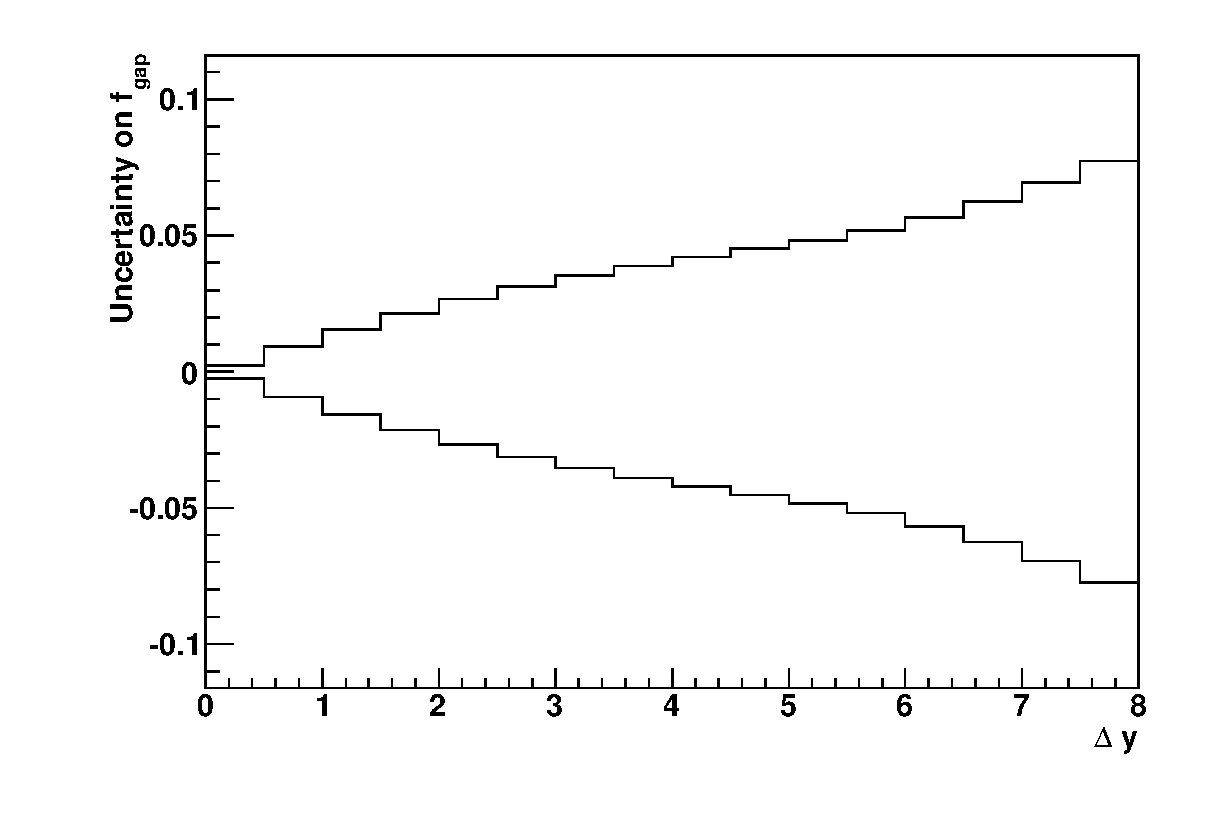
\includegraphics[width=\textwidth]{figures/GBJ2/JES/Smeared__GapFraction_deltaY.eps}
        \end{subfigure}%
        \begin{subfigure}[b]{0.5\textwidth}
                \centering
                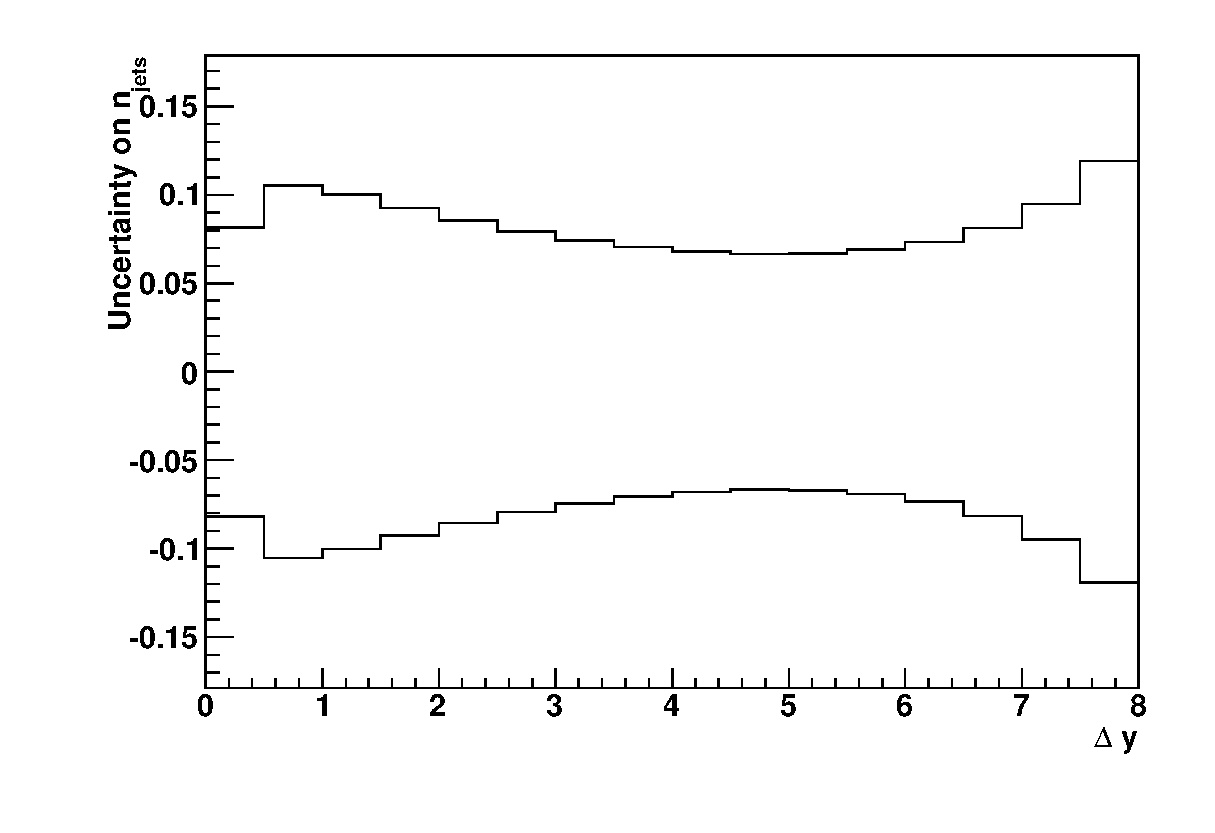
\includegraphics[width=\textwidth]{figures/GBJ2/JES/Smeared__prof_deltaY_njets.eps}
        \end{subfigure}%
\caption[Uncertainty bands due to the JES uncertainty for gap fraction and mean number of jets]{
The uncertainty on the (a) gap fraction and (b) mean number of jets in the rapidity interval due to the JES uncertainty as a function of dijet rapidity separation. 
\label{GBJ2:JES:gap_njets}}
\end{figure}



\begin{figure}
\centering
        \begin{subfigure}[b]{0.5\textwidth}
                \centering
                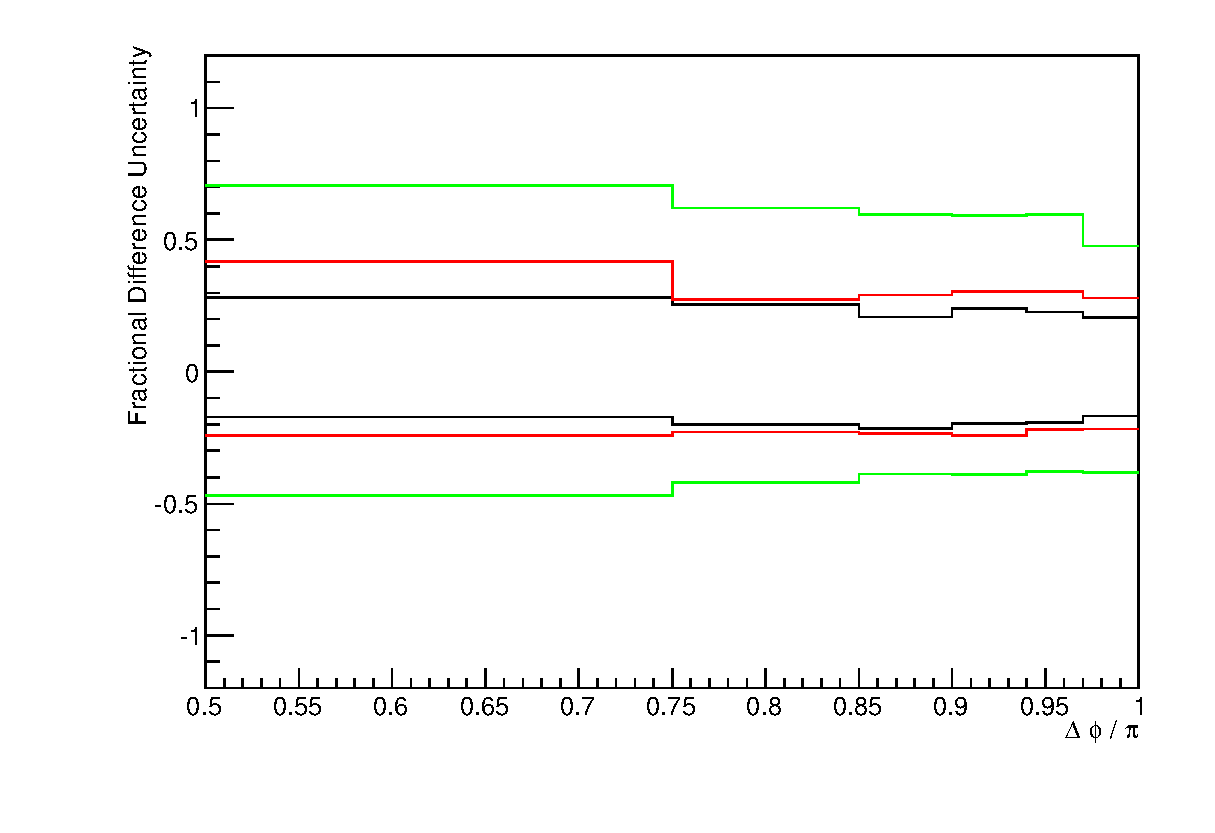
\includegraphics[width=\textwidth]{figures/GBJ2/JES/Smeared__dPhi__7_8.eps}
        \end{subfigure}%
        \begin{subfigure}[b]{0.5\textwidth}
                \centering
                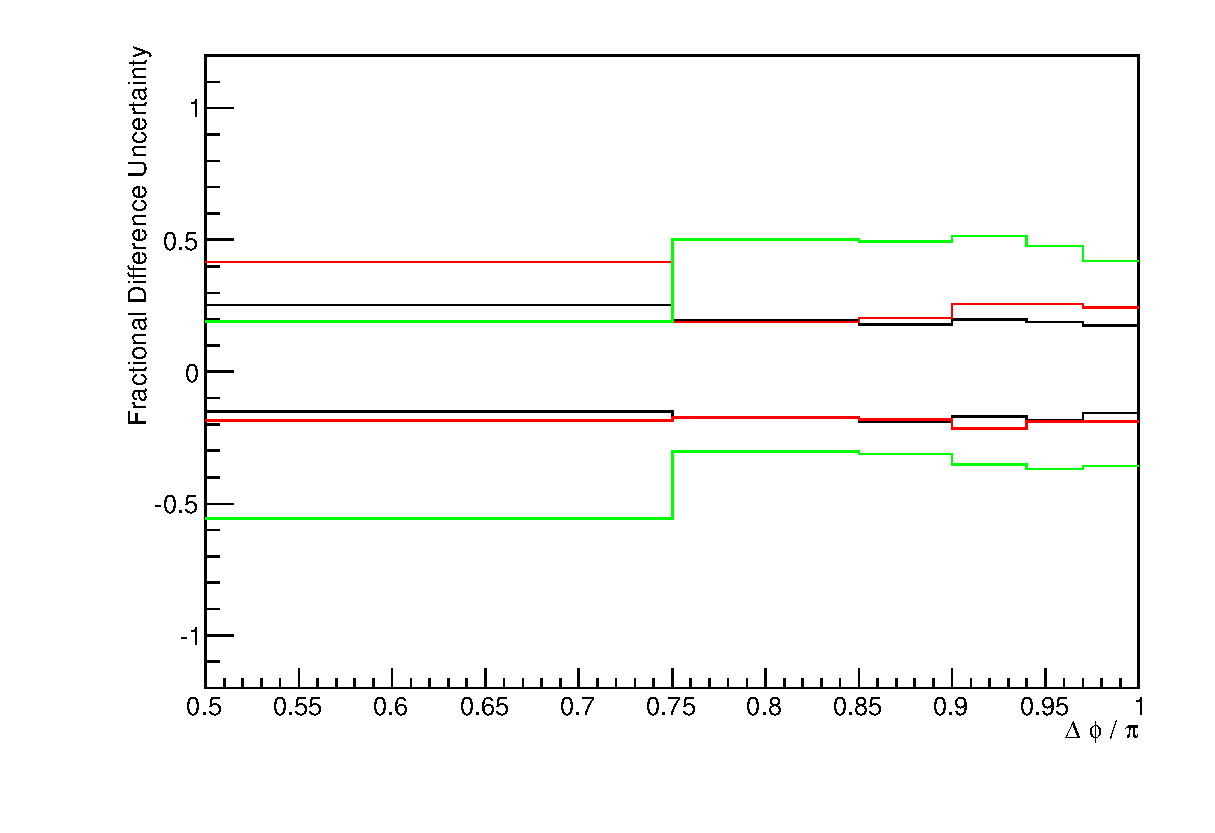
\includegraphics[width=\textwidth]{figures/GBJ2/JES/Smeared__dPhi_gap__7_8.eps}
        \end{subfigure}%
\caption[Uncertainty bands due to the JES uncertainty for \dphiDist{}]{
The uncertainty on \dphiDist{} due to the JES uncertainty for (a) inclusive events and (b) gap events. 
Three dijets rapidity separation slices are shown, $2<\dy{}<3$ in black, $4<\dy{}<5$ in red and $7<\dy{}<8$ in green.
\label{GBJ2:JES:dPhi}}
\end{figure}


\begin{figure}
\centering
        \begin{subfigure}[b]{0.5\textwidth}
                \centering
                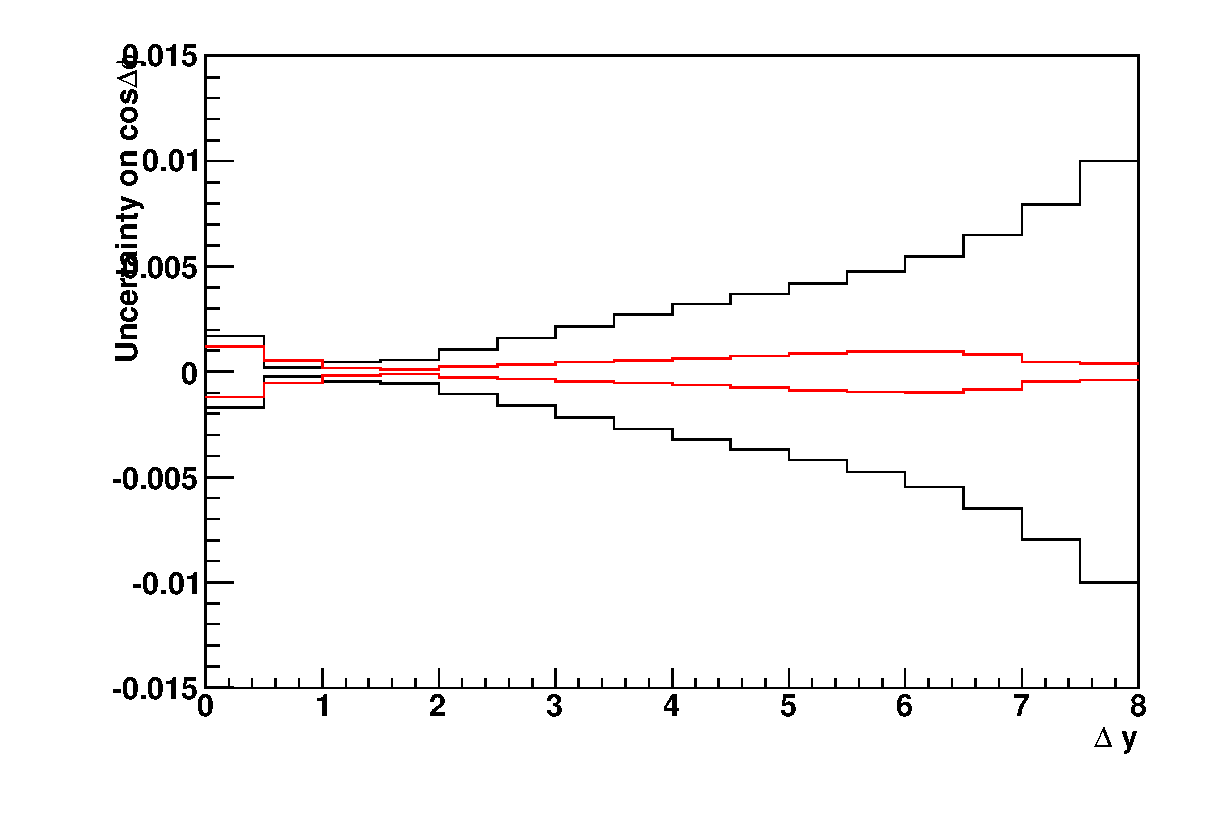
\includegraphics[width=\textwidth]{figures/GBJ2/JES/Smeared__cosdPhi_deltaY_gap.eps}
        \end{subfigure}%
        \begin{subfigure}[b]{0.5\textwidth}
                \centering
                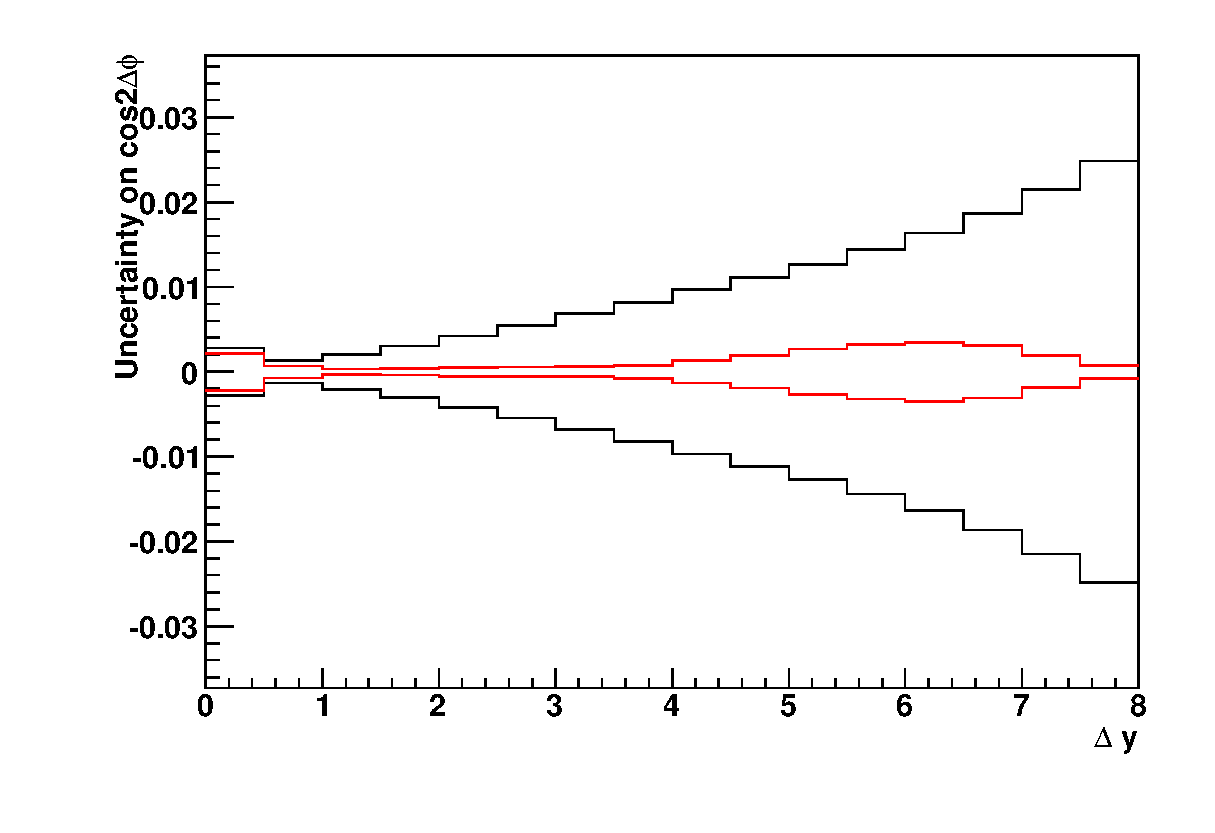
\includegraphics[width=\textwidth]{figures/GBJ2/JES/Smeared__cos2dPhi_deltaY_gap.eps}
        \end{subfigure}%
\caption[Uncertainty bands due to the JES uncertainty for \mean{\cosdphi{}} and  \mean{\costwodphi{}}]{
The shape uncertainty on (a) \mean{\cosdphi{}} and (b) \mean{\costwodphi{}} distributions due to the JES uncertainty as a function of dijet rapidity separation.
The gap events are plotted in red and the inclusive events in black.
\label{GBJ2:JES:cos}}
\end{figure}


\begin{figure}
\centering
        \begin{subfigure}[b]{0.5\textwidth}
                \centering
                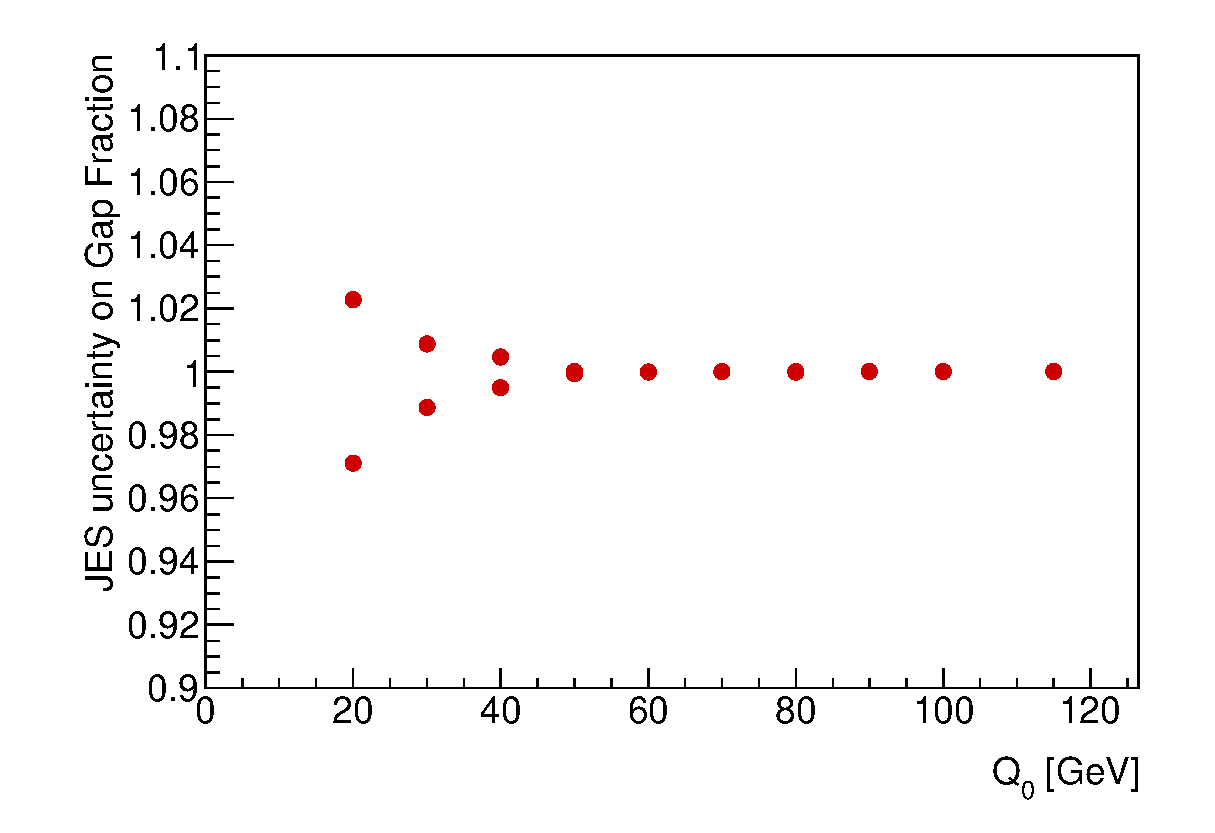
\includegraphics[width=\textwidth]{figures/GBJ2/JES/Smeared2_3__Q0.eps}
        \end{subfigure}%
        \begin{subfigure}[b]{0.5\textwidth}
                \centering
                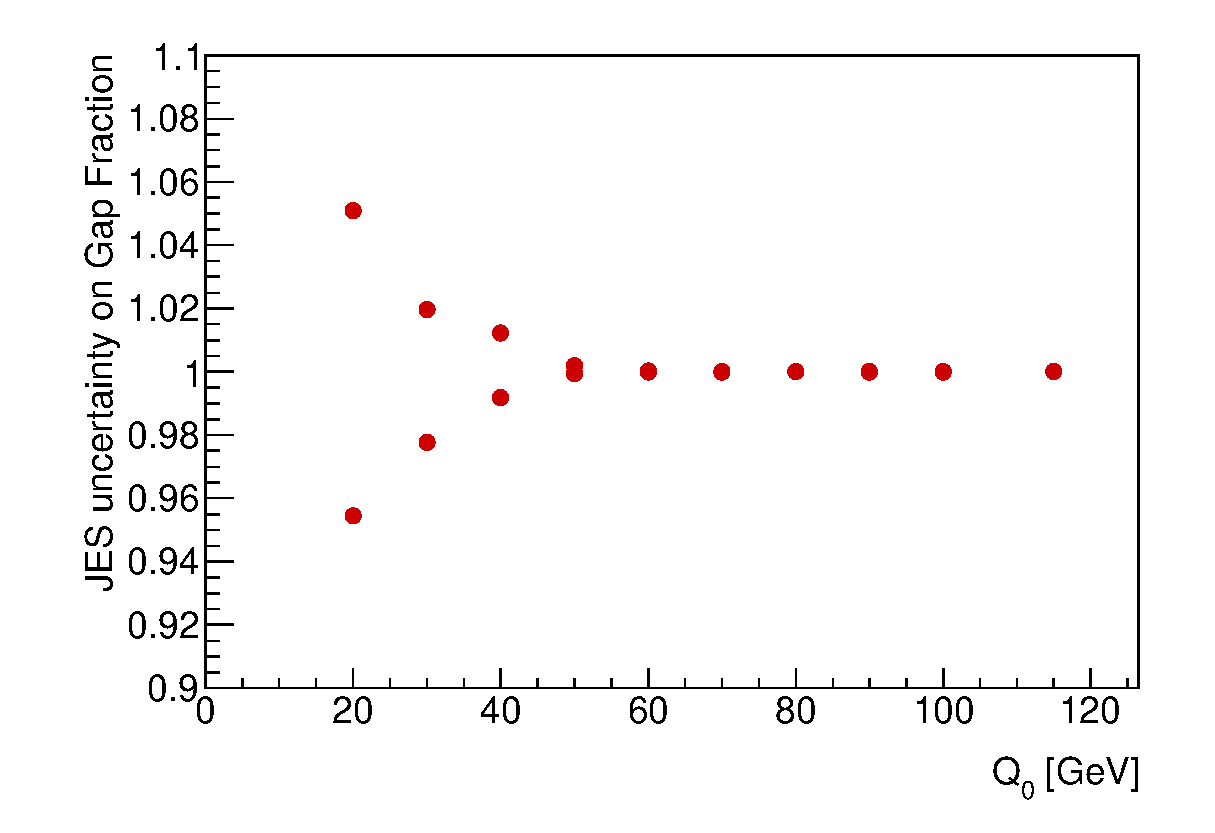
\includegraphics[width=\textwidth]{figures/GBJ2/JES/Smeared4_5__Q0.eps}
        \end{subfigure}%

        \begin{subfigure}[b]{0.5\textwidth}
                \centering
                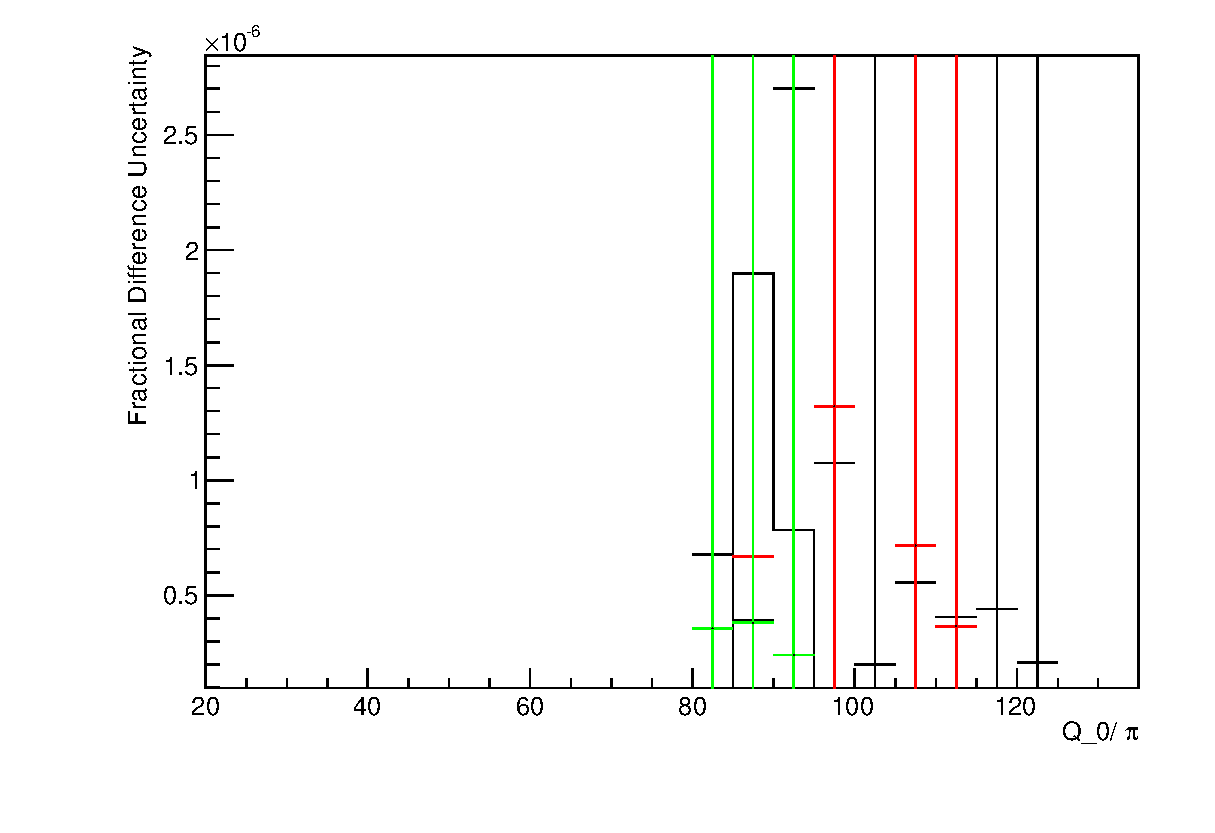
\includegraphics[width=\textwidth]{figures/GBJ2/JES/Smeared7_8__Q0.eps}
        \end{subfigure}%
\caption[Uncertainty bands due to the JES uncertainty for gap fraction as a function of \qz{}]{
The uncertainty on the gap fraction due to the JES uncertainty as a function of \qz{} for dijet rapidity separation (a) $2<\dy{}<3$, (b) $4<\dy{}<5$, and (c) $7<\dy{}<8$.
\label{GBJ2:JES:Q0}}
\end{figure}
